\documentclass[../../main.tex]{subfiles}

\begin{document}

\hyphenation{par-ti-cu-la-res}

\section{Circuitos integradores y derivadores}

Algunas aplicaciones \'utiles de circuitos con amplificadores operacionales implican realizar operaciones matem\'aticas entre las se\~nales involucradas en un circuito. En esta secci\'on estudiaremos los casos particulares de derivaci\'on e integraci\'on con \textit{op amps}. En ambos circuitos, se utilizar\'a el operacional \textit{LM833}, as\'i como una resistencia de $R = 15k\Omega$ y un capacitor de $C = 6.8nF$.

\subsection{An\'alisis matem\'atico} \label{ssection:formulas}

Dado que todos los circuitos estudiados en esta secci\'on presentan la misma topolog\'ia general, analizaremos el caso general para cada modelo de operacional, y para obtener los resultados particulares bastar\'a reemplazar en el resultado final con los valores de $Z_1$ y $Z_2$ que corresponda.

\begin{figure} [H]
	\centering
	\begin{circuitikz}
  		\draw (0,0) node[op amp] (opamp) {}
  		(opamp.-) to [generic, l_=$Z_1$, *-o] ($(opamp.-)-(2,0)$) node[left]{$V_{in}$}
  		(opamp.-) |- ($(opamp.-)+(0.2,1)$) to[generic, l=$Z_2$] ($(opamp.-)+(2.2,1)$) -|
  		(opamp.out) to[short,*-] ($(opamp.out)+(.5,0)$) node [right] {$V_{out}$} node [ocirc] {} 
  		(opamp.+) to[short] ($(opamp.+) - (0,.5)$) node[ground] {}
		  ;
		\end{circuitikz}
	\caption{Circuito inversor}
\end{figure}

\subsubsection{$A_0$ infinito}
Si consideramos que $V^-=V^+$, entonces este circuito presenta una tierra virtual en ese punto, y por lo tanto puede resolverse trivialmente, obtieniendo:

\begin{equation} \label{eq:tf-ideal} H(s) = -\frac{Z_2(s)}{Z_1(s)} \end{equation}
\begin{equation} \label{eq:zin-ideal} Z_{in}(s) = Z_1(s) \end{equation}


\subsubsection{$A_0$ finito}
Al considerar que la ganancia no es infinita, ya no se cumple que $V^-=0$, aunque mientras que sigamos admitiendo que la impedancia del operacional es infnita, existe una sola corriente en el circuito. Por lo tanto las ecuaciones quedan planteadas como:

 \[
	\left\{
 	\begin{array}{ll}
		V_{in} - V_{out} = I\cdot (Z_1+Z_2)\\
		V^- = V_{out} + I\cdot Z_2\\
		V_{out} = - A_0 \cdot V^-
	\end{array}
	\right.
 \]

En este caso, el resultado obtenido es:
\begin{equation} \label{eq:tf-ao} H(s) =-\frac{A_0\cdot Z_2}{Z_2+(A_0+1)\cdot Z_1} 
						\sim-\frac{A_0\cdot Z_2}{Z_2+A_0\cdot Z_1}  \end{equation}
\begin{equation} \label{eq:zin-ao} Z_{in}(s) = \frac{Z_2}{A_0+1} +Z_1 \sim  \frac{Z_2}{A_0} +Z_1 \end{equation}

Podemos verificar la validez de estas expresiones notando que $\lim_{A_0\to\infty}$ llegamos, en ambos casos, a los resultados de la secci\'on anterior.\par

Para el operacional utilizado, el valor de $A_0$ es $110dB$.

\subsubsection{$A_{vol}(s)$}
Para obtener la f\'ormula del modelo de polo dominante aplicado a este circuito, basta reemplazar $A_0$ por $A_{vol}(s)=\frac{A_0}{\frac{s}{\omega_p} +1}$ en las ecuaciones \ref{eq:tf-ao} y \ref{eq:zin-ao}. Se obtiene entonces:

\begin{equation} \label{eq:tf-avol} H(s) =-\frac{A_0\cdot Z_2}{\left(\frac{s}{\omega_p}+1\right)\left(Z_2+Z_1\right) + A_0 \cdot Z_1}  \sim
- \left(\frac{A_0 \cdot Z_2}{A_0 \cdot Z_1 + Z_2}\right) \cdot \left(\frac{1}{\left(\frac{Z_1 + Z_2}{A_0 \cdot Z_1 + Z_2} \cdot \frac{1}{\omega_p}\right) \cdot s + 1}\right)
\end{equation}
\begin{equation} \label{eq:zin-avol} Z_{in}(s) = \frac{\left(\frac{s}{\omega_p}+1\right)\left(Z_2+Z_1\right)+ A_0 \cdot Z_1}{\frac{s}{\omega_p}+A_0+1}
\sim \left(\frac{Z_2 + A_0 \cdot Z_1}{A_0}\right) \cdot \left(\frac{ \left(\frac{Z_1+Z_2}{Z_2+A_0\cdot Z_1}\right)\cdot \frac{1}{\omega_p} \cdot s + 1 }{ \frac{1} {A_0 \cdot \omega_p} \cdot s + 1}\right) \end{equation}

En este caso tambi\'en se verifica que el t\'ermino que no depende de $\omega_p$ tiende a la ganancia cuando $A_0$ tiende a infinito. Sin embargo, se agrega un polo a la transferencia, y un polo y un cero a la impedancia.\par

En el \textit{LM833}, dado que el valor del $BWP = 16MHz$, $\omega_p = 2\pi \frac{BWP}{A_0} \sim 2\pi \cdot 50.6 Hz$.










\subsection{Derivador}

Para armar un circuito derivador con los componentes mencionados, la conexi\'on debe realizarse de la siguiente manera:

\begin{figure} [H]
	\centering
	\begin{circuitikz}
  		\draw (0,0) node[op amp] (opamp) {}
  		(opamp.-) to [C, l_=$C$, *-o] ($(opamp.-)-(2,0)$) node[left]{$V_{in}$}
  		(opamp.-) |- ($(opamp.-)+(0.2,1)$) to[R=$R$] ($(opamp.-)+(2.2,1)$) -|
  		(opamp.out) to[short,*-] ($(opamp.out)+(.5,0)$) node [right] {$V_{out}$} node [ocirc] {} 
  		(opamp.+) to[short] ($(opamp.+) - (0,.5)$) node[ground] {}
  ;
\end{circuitikz}
	\caption{Circuito derivador}
\end{figure}


\subsubsection{An\'alisis matem\'atico: respuesta en frecuencia}

Si consideramos el modelo ideal para el \textit{op amp}, al tener una tierra virtual en $V^-$, la entrada y la salida est\'an aisladas entre s\'i, reemplazando en \ref{eq':tf-ideal} $Z_1=\frac{1}{sC}$ y $Z_2=R$:

\[ H(s) = -RC \cdot s \]

Antitransformando esta expresi\'on, obtenemos que $v_{out}(t) = -RC \cdot \frac{\partial}{\partial t}v_{in}(t)$, con lo cual anal\'iticamente podemos ver que cumple la funci\'on planteada inicialmente, si bien la salida estar\'a invertida y multiplicada por una constante.  \par

Con el modelo de $A_0$ constante, en cambio, la ecuaci\'on resultante es:

\[ H(s) = -\left(\frac{A_0 \cdot RC}{1+A_0}\right) \cdot \left(\frac{s}{ \left(\frac{RC}{A_0+1}\right) \cdot s + 1\ }\right)\]

Dado que $A_0+1\sim A_0$, la constante es pr\'acticamente id\'entica a la del modelo ideal, pero en este caso se agrega a la transferencia un polo en $f= \frac{A_0+1}{2\pi \cdot RC} \sim 493MHz$. Por lo tanto, sus efectos no ser\'ian apreciables hasta llegar a frecuencias en el orden de los $MHz$, con lo cual hasta frecuencias de $kHz$ el circuito deber\'ia derivar correctamente.

Por \'ultimo, teniendo en cuenta el polo dominante del operacional, la funci\'on transferencia queda reducida a:

\[ H(s) = -\left(\frac{A_0 \cdot RC}{1+A_0}\right) \cdot 
	\left( \frac{s} { \left( \frac{RC}{(1+A_0)\cdot \omega_p} \right)\cdot s^2 + \left( \frac{RC\cdot \omega_p +1}{(1+A_0)\cdot\omega_p} \right)\cdot s + 1  } \right) \]
	
En este caso, el polo queda de segundo orden, con $f_0 = \frac{1}{2\pi} \sqrt{\frac{(1+A_0)\cdot \omega_p}{RC}} = 158kHz$, con $\xi = \frac{\omega_0 \cdot (RC\cdot\omega_p+1)} {2\omega_p\cdot(1+A_0)} = 0.005$. La respuesta en frecuencia, entonces, presentar\'a un sobrepico considerable en esta frecuencia, y un salto abrupto de $-180^\circ$ en la fase. Sin embargo, aqu\'i no se est\'an teniendo en cuenta los $50\Omega$ de impedancia del generador de funciones que quedar\'an en serie con el circuito, que provocar\'ian que el sobrepico no sea tan pronunciado. Esto se tratar\'a m\'as en detalle en la secci\'on \ref{ssection:dcomp}. \par

Como el \'ultimo modelo introduce un cambio tan grande en el comportamiento del circuito, ser\'a el que contrastaremos con los resultados. Se espera que el circuito derive se\~nales con frecuencia menor a la del polo. El alto factor de calidad sugerir\'ia que no se empezar\'ian a observar cambios hasta frecuencias del mismo orden que ella.



\subsubsection{An\'alisis matem\'atico: impedancia de entrada}

Idealmente, la impedancia de entrada del circuito ser\'ia solo la del capacitor. Si utiliz\'azemos la expresi\'on \ref{eq:zin-ao}, deber\'iamos adem\'as sumar $\frac{R}{A_0}\sim 0.05\Omega$, pero esto ser\'ia comparable con la impedancia del capacitor s\'olo en frecuencias del orden de los $100MHz$, con lo cual despreciaremos su aporte.\par
	
Con el modelo de $A_{vol}(s)$, la funci\'on que se obtiene es:

\[ Z_{in}(s) = \frac{1}{sC} \cdot \left( \frac{ \frac{RC}{(1+A_0)\cdot \omega_p} \cdot s^2 + \frac{1 + RC \cdot \omega_p}{(A_0+1) \cdot \omega_p} \cdot s + 1 }{\frac{1}{(1+A_0)\cdot\omega_p}\cdot s+1 } \right)\]	

Al igual que la transferencia, esta funci\'on tiene $f_0 = 158kHz$ con un $\xi = 0.05$, pero en este caso en un cero en lugar de un polo. El polo que s\'i presenta esta funci\'on est\'a en $16MHz$. 



\subsubsection{An\'alisis de resultados: respuesta en frecuencia} \label{ssection:d-hf}

\begin{figure}  [H]
	\centering
	\label{fig:d-hf}
	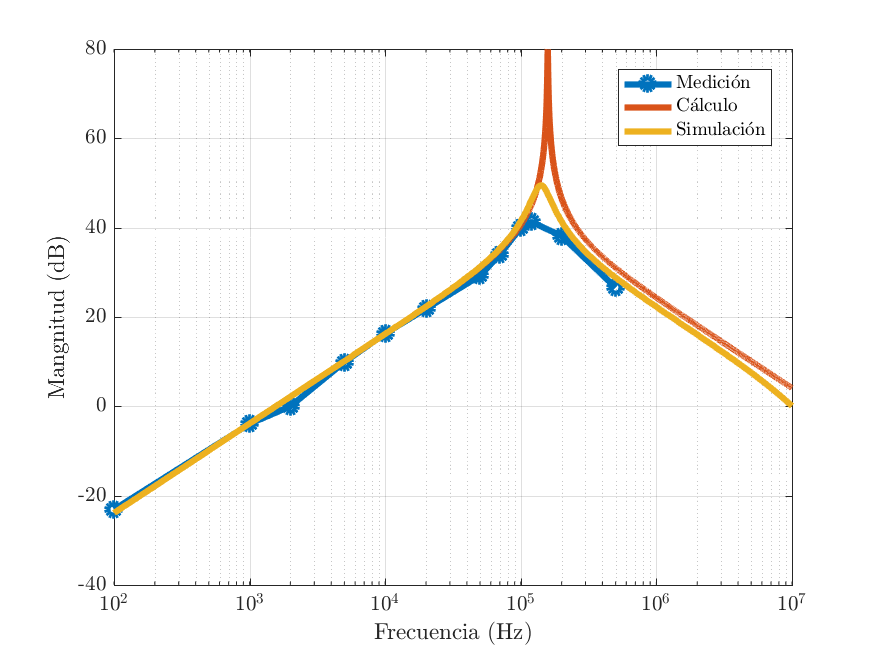
\includegraphics[scale=0.7]{fotos/tc_tp2_ej4_d_Hf_mag.png}
	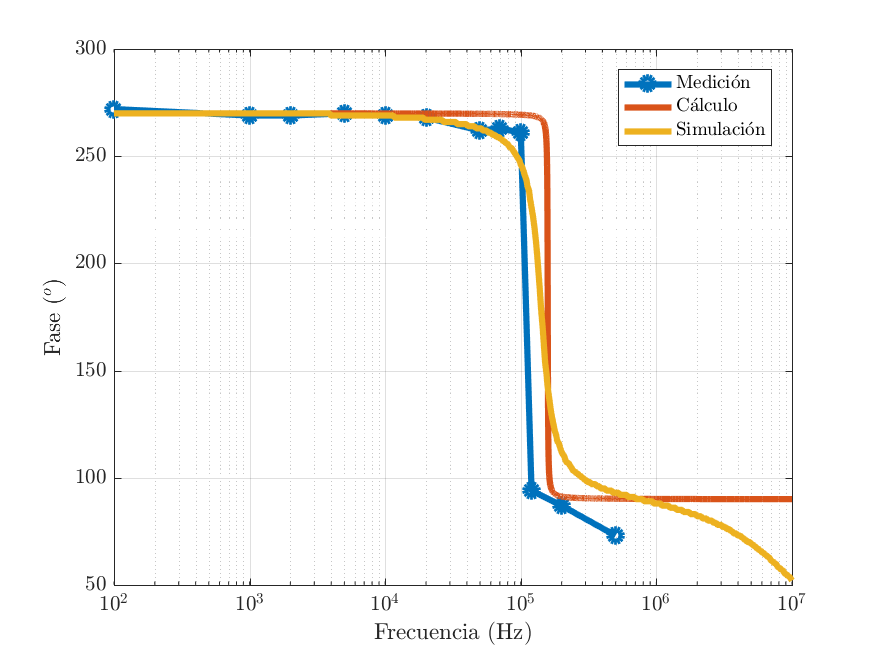
\includegraphics[scale=0.7]{fotos/tc_tp2_ej4_d_Hf_fase.png}
	\caption{Respuesta en frecuencia del derivador}
\end{figure}

En la figura anterior, se observa que el modelo logr\'o precedir correctamente la frecuencia del polo de segundo orden, as\'i como la presencia de un sobre pico. Sin embargo, no se pudo medir en frecuencias muy cercanas a este punto, debido a limitaciones del \textit{slew rate} de $7\frac{V}{\mu s}$ del operacional. A $158k\Omega$, si estimamos que la ganancia ser\'ia de $50dB$ como calcula el simulador, la m\'axima tensi\'on de entrada admisible ser\'ia de $V_{in} = \frac{7\frac{V}{\mu s}}{2\pi \cdot 150kHz \cdot 10^{50/20}}\sim 22mV$, lo cual es del orden del ruido del osciloscopio y por lo tanto no ser\'ia una medici\'on confiable.\par

Observando el comportamiento de la fase, podemos estimar que la predicci\'on del simulador es mejor que la anal\'itica. El hecho de que la fase contin\'ua decreciendo m\'as all\'a de los $90^\circ$ sugerir\'ia que hay otra singularidad en el sistema, que proviene de alg\'un par\'ametro del operacional que el simulador tiene en cuenta y nosotros no. Puesto que la \textit{data sheet} informa que la frecuencia en la cual el operacional tiene ganancia unitaria es $9MHz$, en lugar de los 16 que indicar\'ia el \textit{bandwidth product}, es razonable suponer que el operacional tiene otro polo de frecuencia mucho mayor a la del primero, que llega a apreciarse debido a que se est\'a trabajando a frecuencia y ganancia elevadas.\par 

Otra informaci\'on que se puede extraer de la fase es el rango de frecuencias donde el circuito deriva. La fase se mantuvo en el rango $(-90\pm 3)^\circ$ hasta $f = 20kHz$. M\'as all\'a de ese punto, se considera que no se puede utilizar el circuito como derivador. 



\subsubsection{An\'alisis de resultados: impedancia de entrada}

\begin{figure}  [H]
	\centering
	\label{fig:d-zin}
	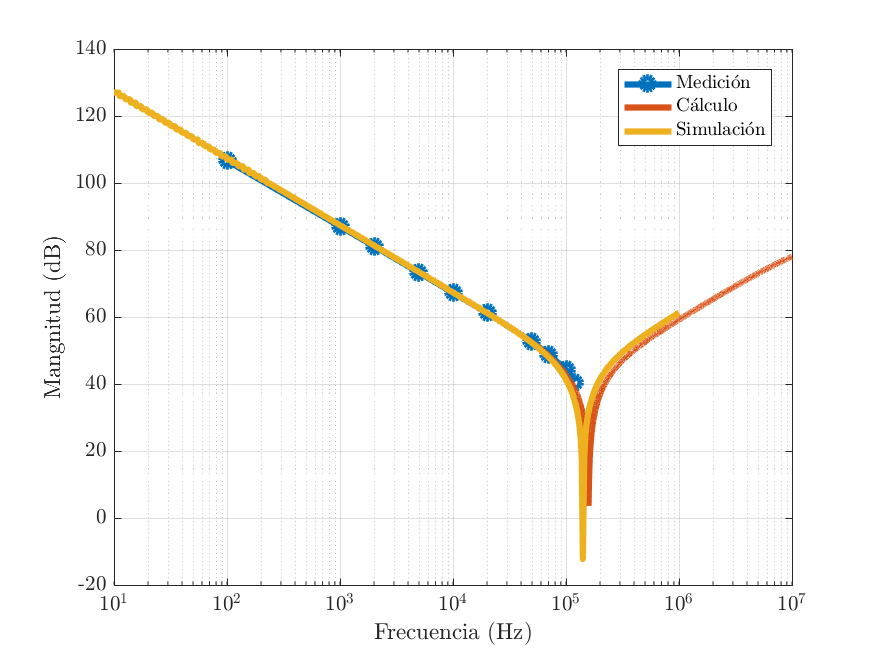
\includegraphics[scale=0.7]{fotos/tc_tp2_ej4_d_Zin_mag.png}
	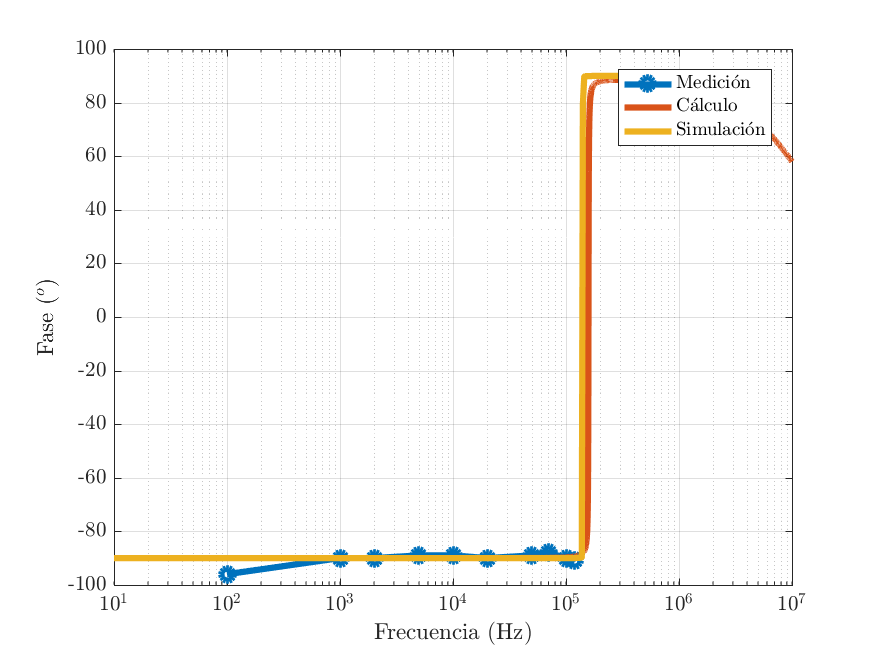
\includegraphics[scale=0.7]{fotos/tc_tp2_ej4_d_Zin_fase.png}
	\caption{Impedancia de entrada del derivador compensado}
\end{figure}

Estas mediciones se realizaron colocando una resistencia de $10k\Omega$ en serie con el circuito, y asumiendo que la misma no introduce cambios de fase en el rango de frecuencias donde se trabaj\'o. \par

Para el rango de frecuencias medido, el comportamiento es pr\'acticamente id\'entico al ideal: la fase se mantiene constante en $-90^\circ$, y la magnitud baja $20dB$ por d\'ecada. No se pudieron hacer mediciones m\'as all\'a de los $120kHz$ debido a las limitaciones explicadas en la secci\'on anterior. En la \'ultima medici\'on se llega a apreciar que el descenso en magnitud es m\'as abrupto, lo cual coincidir\'ia con la presencia del cero de orden dos que se observa en la teor\'ia y en Spice. \par

Si asumimos que la impedancia medida es puramente capacitiva, podemos calcular para cada medici\'on $C = (2\pi \cdot f \cdot 10^{\abs{H}/20})^{-1}$. Salvo para el \'utimo punto, se obtienen valores de $C$ entre 6.9 y $9nF$. Siendo que el valor del capacitor utilizado era $6.8nF\pm 5\%$,  estos valores indicar\'ian que una parte de la impedancia proviene de otros elementos, pero de todas formas el orden de magnitud es el adecuado. Para la \'ultima medici\'on, sin embargo, se obtiene $C=12.4pF$. Esto refuerza la idea de que en esta medici\'on influye el cero de segundo orden proveniente del polo del operacional.


\subsubsection{An\'alisis de resultados: respuesta transitoria}

Seg\'un lo medido en la secci\'on \ref{ssection:d-hf}, deber\'ian poder derivarse se\~nales de $f\leq 20kHz$. 

\begin{figure}  [H]
	\centering
	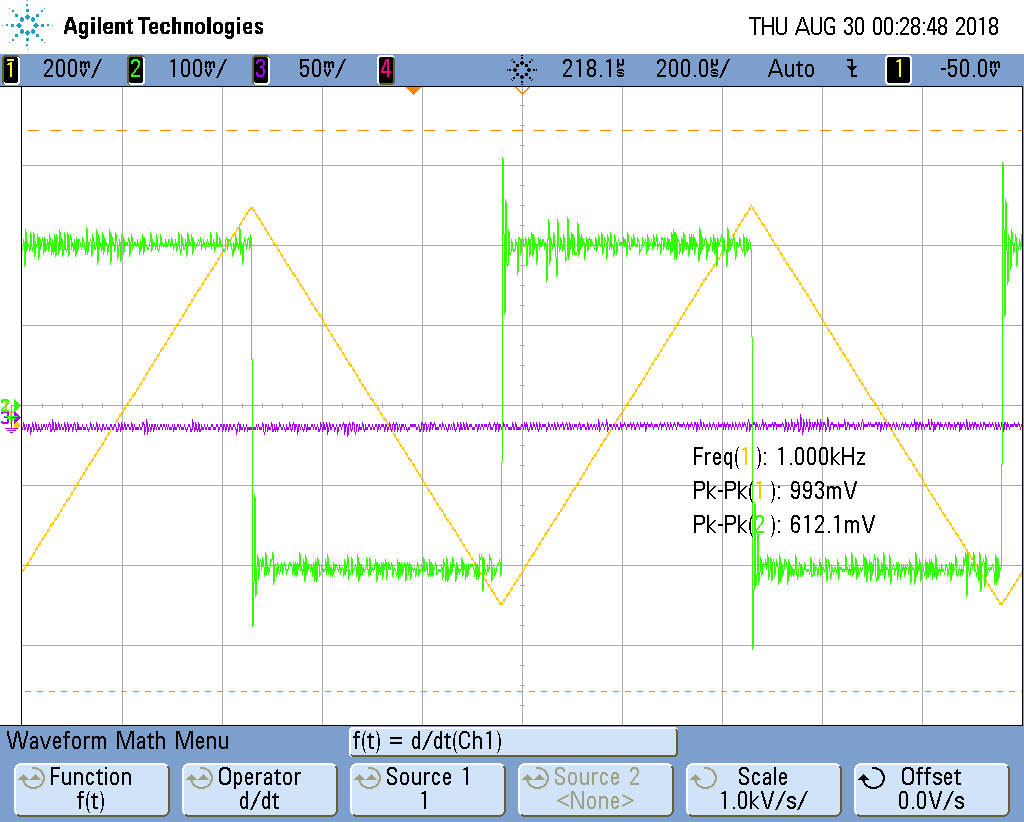
\includegraphics[scale=0.4]{fotos/tc_tp2_ej4_d_1k.png}
	\caption{Respuesta del derivador (verde) a una entrada triangular (amarilla) de $1kHz$}
\end{figure}

Aqu\'i se observa que el circuito deriva correctamente la se\~nal de entrada. Cabe aclarar que la salida se muestra invertida para que se aprecie el efecto derivador, pues como ya se mencion\'o la salida est\'a multiplicada por $(-1)$. \par

Algo que llama la antenci\'on en esta foto son los picos cuando la pendiente de la entrada cambia de signo.


\begin{figure}  [H]
	\centering
	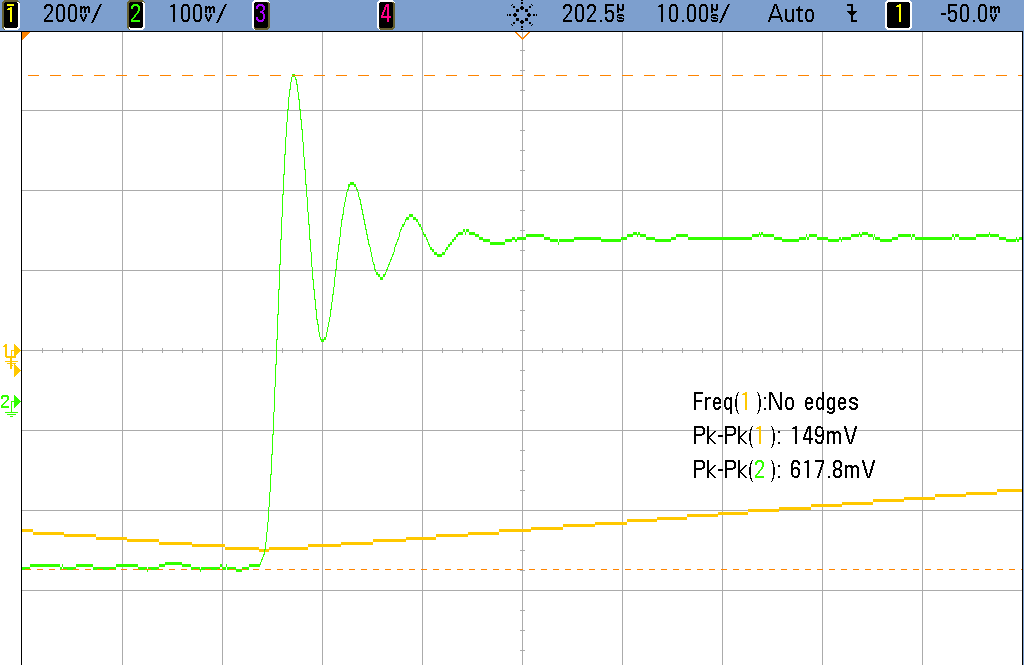
\includegraphics[scale=0.4]{fotos/tc_tp2_ej4_d_1k_transitorio.png}
	\caption{Respuesta transitoria del derivador (verde) a una entrada triangular (amarilla) de $1kHz$}
\end{figure}

Se observa que el circuito oscila antes de estabilizarse. Esto es consistente con el hecho de que los polos del sistema son complejos conjugados, es decir, con que el sistema es subamortiguado.\par


Cuando observamos, en cambio, la respuesta de una frecuencia donde la fase ya no es cercana a $-90^\circ$, la salida no coincide con la derivada de la entrada. Esto tambi\'en puede explicarse con que, como se observa en la figura \ref{fig:d-50k}, el circuito no llega a estabilizarse en un per\'iodo y s\'olo se observa la respuesta transitoria. 

\begin{figure}  [H]
	\centering
	\label{fig:d-50k}
	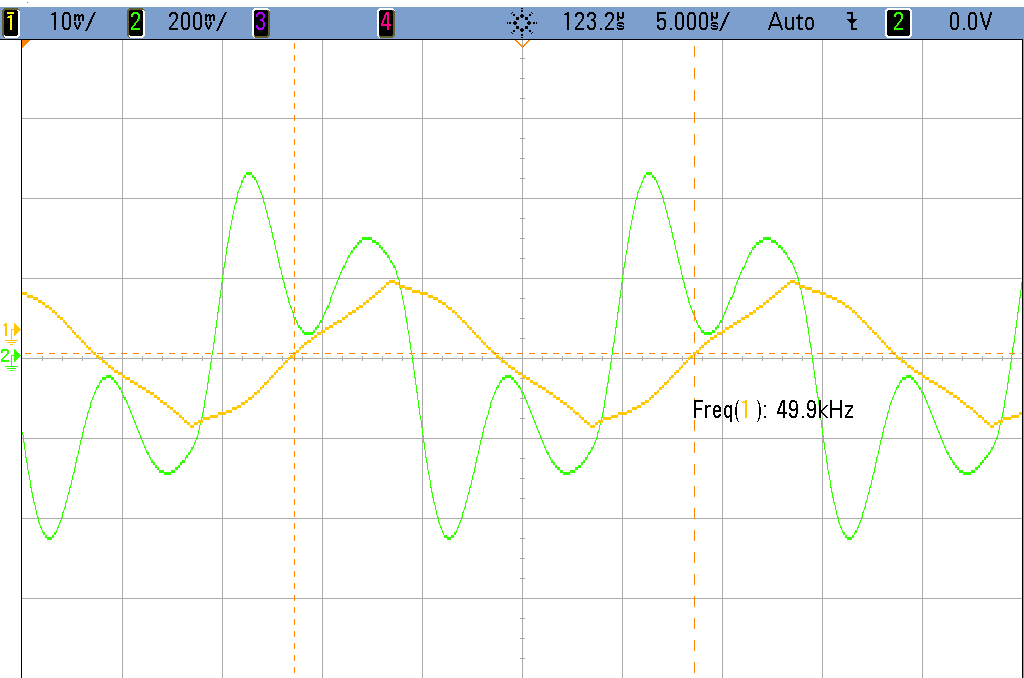
\includegraphics[scale=0.4]{fotos/tc_tp2_ej2_d_50k.png}
	\caption{Respuesta del derivador (verde) a una entrada triangular (amarilla) de $50kHz$}
\end{figure}




\subsection{Derivador compensado} \label{ssection:dcomp}
En la secci\'on anterior, la elevada ganancia del sistema en la frecuencia del polo impidi\'o que se pudiesen tomar mediciones en un gran rango de frecuencia. Por lo tanto, procederemos a continuaci\'on a compensar este comportamiento.\par

Si observamos la funci\'on transferencia ideal del circuito derivador, observamos que la ganancia se hace infinita cuando la frecuencia tambi\'en tiende a infinito. Esto se debe a que el sistema presenta un cero en el origen, que proviene de que para frecuencias altas la impedancia del capacitor disminuye y tiende a cero. Esto puede solucionarse imponiendo una impedancia m\'inima independiente de la frecuencia, lo cual se puede lograr colocando un resistor en serie con el capacitor.\par 

\begin{figure} [H]
	\centering
	\begin{circuitikz}
  		\draw (0,0) node[op amp] (opamp) {}
  		(opamp.-) to [C, l_=$C$, *-o] ($(opamp.-)-(2,0)$) 
		to [R, l_=$R_C$, *-o]  ($(opamp.-)-(4,0)$) node[left]{$V_{in}$}
  		(opamp.-) |- ($(opamp.-)+(0.2,1)$) to[R=$R$] ($(opamp.-)+(2.2,1)$) -|
  		(opamp.out) to[short,*-] ($(opamp.out)+(.5,0)$) node [right] {$V_{out}$} node [ocirc] {} 
  		(opamp.+) to[short] ($(opamp.+) - (0,.5)$) node[ground] {}
  ;
\end{circuitikz}
	\caption{Circuito derivador compensado}
\end{figure}

\subsubsection{An\'alisis matem\'atico: respuesta en frecuencia}
El an\'alisis de este circuito es equivalente al efectuado en la secci\'on \ref{ssection:formulas}, efectuando las sustituciones  $Z_1=R_C+\frac{1}{sC}$ y $Z_2 = R$. 

La funci\'on transferencia que se obtiene es:

\begin{equation} H(s) = -\left(\frac{A_0 \cdot RC \cdot s}{1+A_0}\right) \cdot
\left(\frac{1}{ \frac{(R+R_C)\cdot C}{(1+A_0)\cdot \omega_p} \cdot s^2 + [\frac{1}{\omega_p}+ C\cdot(R+R_C\cdot(1+A_0))]\cdot \frac{1}{1+A_0} \cdot s + 1 }\right)\end{equation}

Por lo tanto, para eliminar el sobrepico debemos obtener el valor de $R_C$ tal que $xi\geq 0.707$. Esto se resolvi\'o con el siguiente c\'odigo en \textit{Matlab}:\\
\code{r = 15e3; c = 6.8e-9;}\newline
\code{Ao = 10\^(110/20); \% de la hoja de datos: Ao=110dB}\\
\code{BWP = 16e6;}\\
\code{wp = 2*pi*BWP/Ao;}\\
\\
\code{syms r2;}\\
\code{w0 = sqrt(wp*(1+Ao)/c/(r+r2));}\\
\code{xi = w0/2*(c*(r+r2*(1+Ao))+1/wp)/(1+Ao);}\\
\code{r2 = eval(solve(xi == 0.707, r2));}

Se obtiene as\'i que $R_C \geq 210\Omega$. Sin embargo, si se tomase la m\'inima indispensable para quitar el sobrepico, se tendr\'ia una ganancia de aproximadamente $40dB$ en la frecuencia del polo. Por lo tanto, se utiliz\'o $R_C = 470\Omega$, con la cual la magnitud no deber\'ia superar los $30dB$. \par

Como ahora el sistema esta sobreamortiguado, los polos ya no son complejos conjugados sino dos polos reales distintos. Calculando $\omega_0$ y $\xi$ con el valor elegido de $R_2$, las frecuencias de corte que se obtienen son 

\subsubsection{An\'alisis matem\'atico: impedancia de entada}
En este caso, la impedancia de entrada ideal es $R_C$ en serie con el capacitor:

\[ H(s) = \frac{1}{C} \cdot \frac{R_C C \cdot s + 1}{s} \]
 
 Esta transferencia cuenta con un polo en el origen y un cero en $f = \frac{1}{2\pi \cdot R_C C} \sim 50kHz$.\par

De igual manera que el caso anterior, se desprecian los $0.05\Omega$ que se suman en el modelo de $A_0$ constante.\par

Considerando, en cambio, el modelo de polo dominante, la impedancia de entrada que se obtiene es:

\begin{equation}Z{in}(s) = \frac{1} {s \cdot C} \cdot \left(\frac{ \frac{(R+R_C)\cdot C}{\omega_p}\cdot s^2 +  [\frac{1}{\omega_p}+ C\cdot(R+R_C\cdot(1+A_0))]\cdot \frac{1}{1+A_0}\cdot s + 1 }{ \frac{1}{(1+A_0)\cdot \omega_p}\cdot s + 1 }\right)\end{equation}

Los ceros de esta funci\'on est\'an en los polos de la transferencia, es decir que tiene un , y se agrega adem\'as un polo en $f_1 =  56kHz$ y $f_2 = 432kHz$. Teniendo en cuenta que se realizar\'an mediciones en ese rango, se utilizar\'a este modelo para comparar con las mediciones.

\subsubsection{An\'alisis de resultados: respuesta en frecuencia}

En este caso s\'i se pudieron efectuar mediciones en un rango continuo de mediciones gracias a la ausencia del sobrepico. Los resultados obtenidos fueron:

\begin{figure}  [H]
	\centering
	\label{fig:dcomp-hf}
	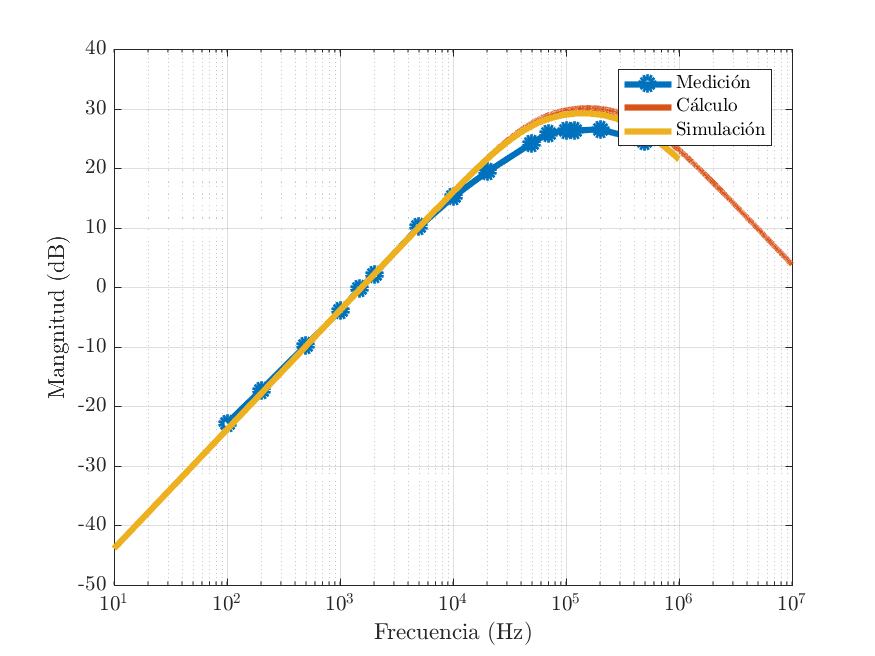
\includegraphics[scale=0.7]{fotos/tc_tp2_ej4_dcomp_Hf_mag.png}
	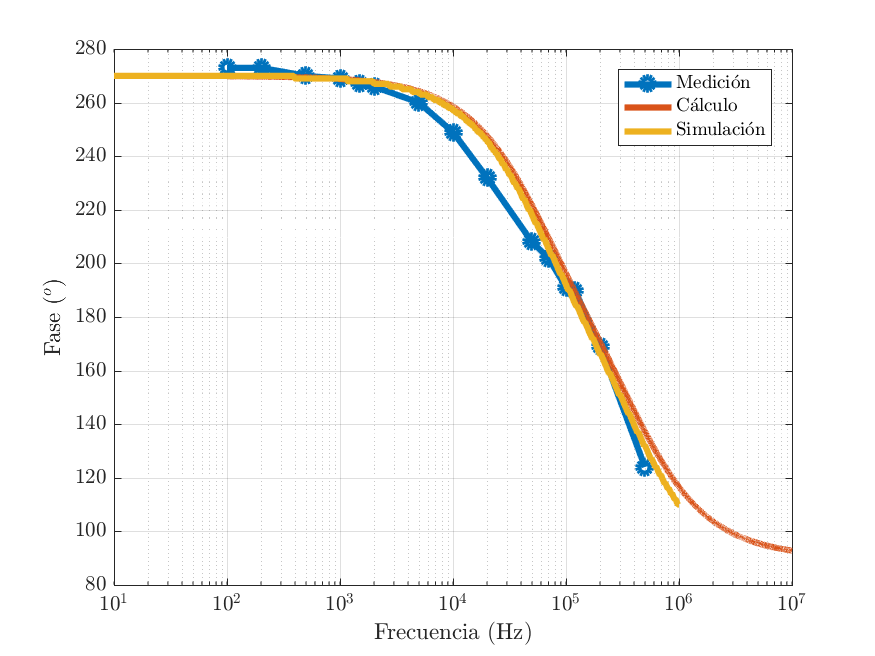
\includegraphics[scale=0.7]{fotos/tc_tp2_ej4_dcomp_Hf_fase.png}
	\caption{Respuesta en frecuencia del derivador compensado}
\end{figure}

El modelo predice adecuadamente el comportamiento del circuito. El hecho de que la magnitud m\'axima medida no coincida con la calculada ni la simulada podr\'ia atribuirse a que las mediciones se realizaron con tasas de cambio de $V_{out}$ cercanas, si bien inferiores, al \textit{slew rate} del operacional. Este efecto se habr\'ia visto exacerbado de haber elegido una resistencia de compensaci\'on menor.\par

En base a los resultados obtenidos para la fase, el nuevo circuito integra hasta $f = 2k\Omega$, es decir un orden de magnitud menos que el derivador no compensado.


\subsubsection{An\'alisis de resutlados: impedancia de entrada}

\begin{figure}  [H]
	\centering
	\label{fig:dcomp-zin}
	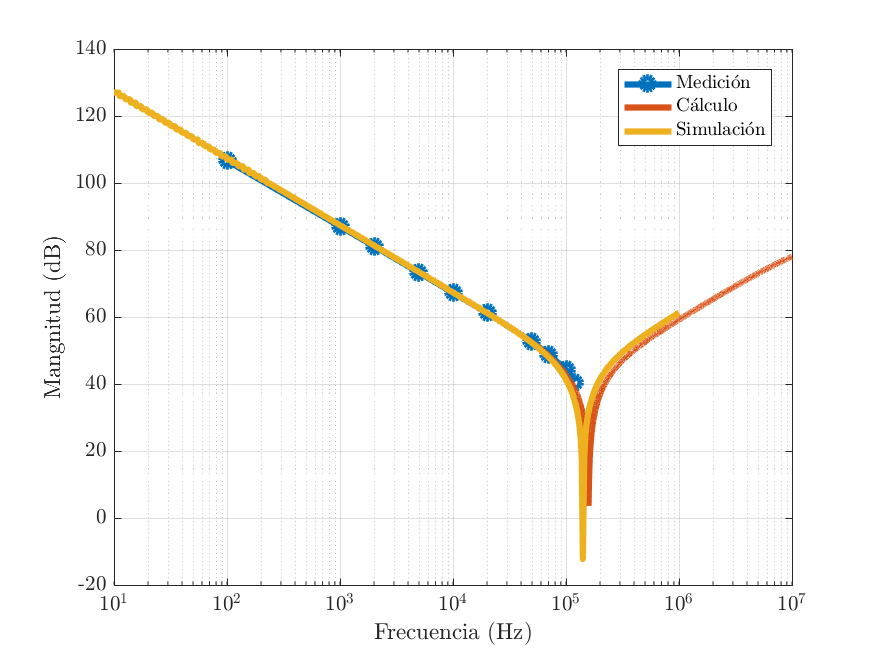
\includegraphics[scale=0.7]{fotos/tc_tp2_ej4_d_Zin_mag.png}
	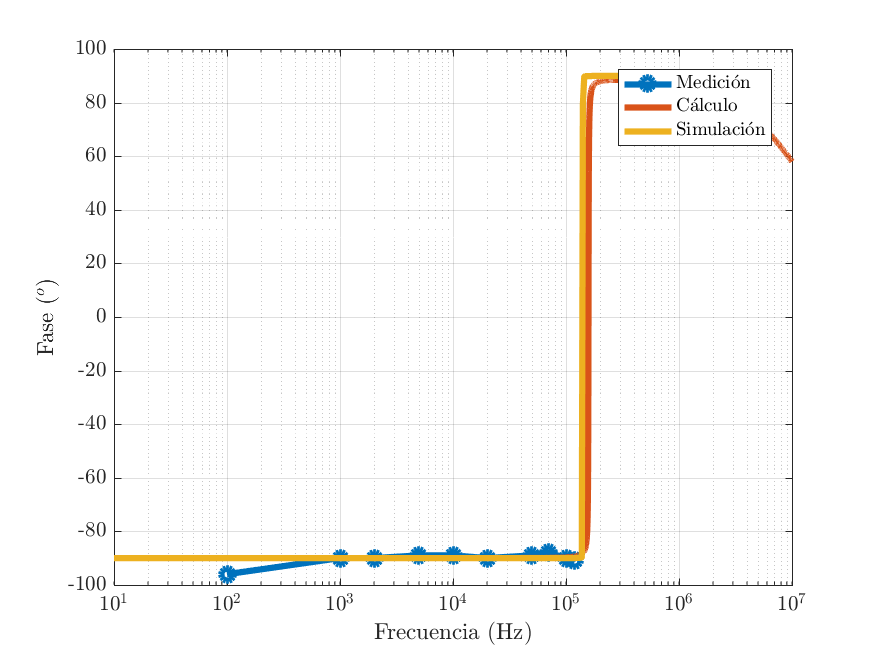
\includegraphics[scale=0.7]{fotos/tc_tp2_ej4_d_Zin_fase.png}
	\caption{Impedancia de entrada del derivador compensado}
\end{figure}


Las mediciones cumplen las predicciones del simulador y las anal\'iticas, que esta vez coinciden entre ellas. Se logr\'o satisfactoriamente lograr limitar el m\'inimo de impedancia de entrada.


\subsubsection{An\'alisis de resultados: respuesta transitoria}

Repetiremos la medici\'on que realizamos para el circuito no compensado en $f=1kHz$.

\begin{figure}  [H]
	\centering
	\label{fig:dcomp-1k}
	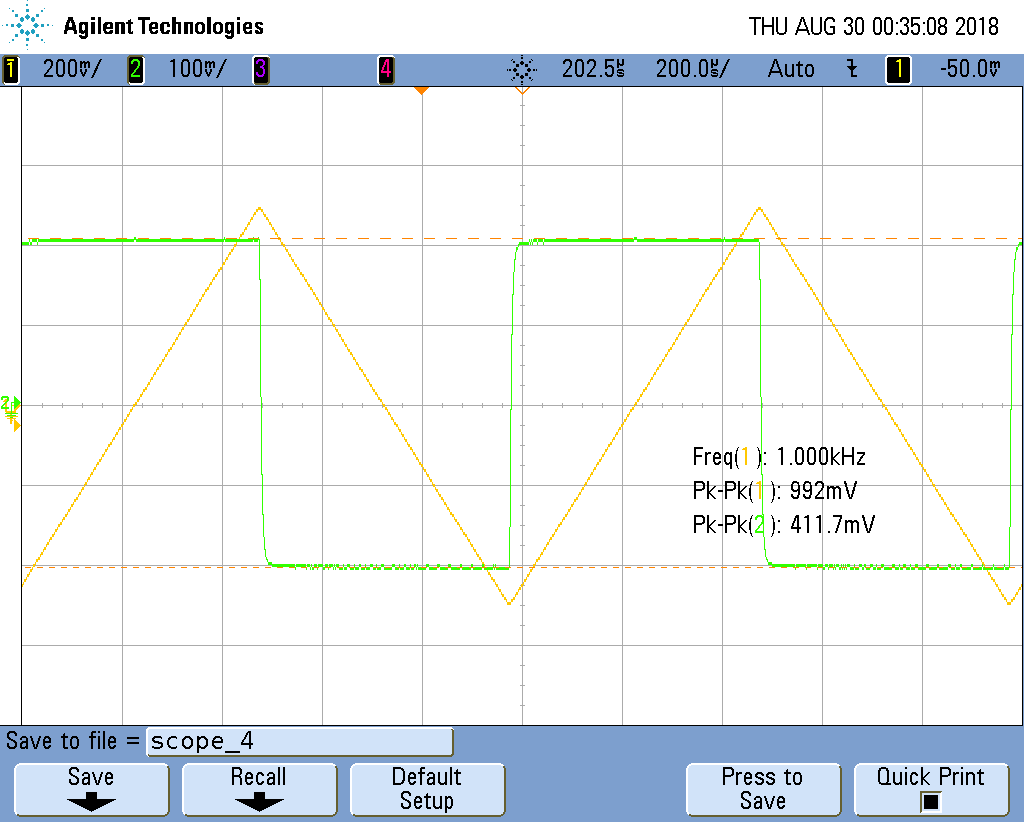
\includegraphics[scale=0.4]{fotos/tc_tp2_ej4_dcomp_1k.png}
	\caption{Respuesta del derivador compensado (verde) a una entrada triangular (amarilla) de $1kHz$}
\end{figure}

\begin{figure}  [H]
	\centering
	\label{fig:dcomp-1k-trans}
	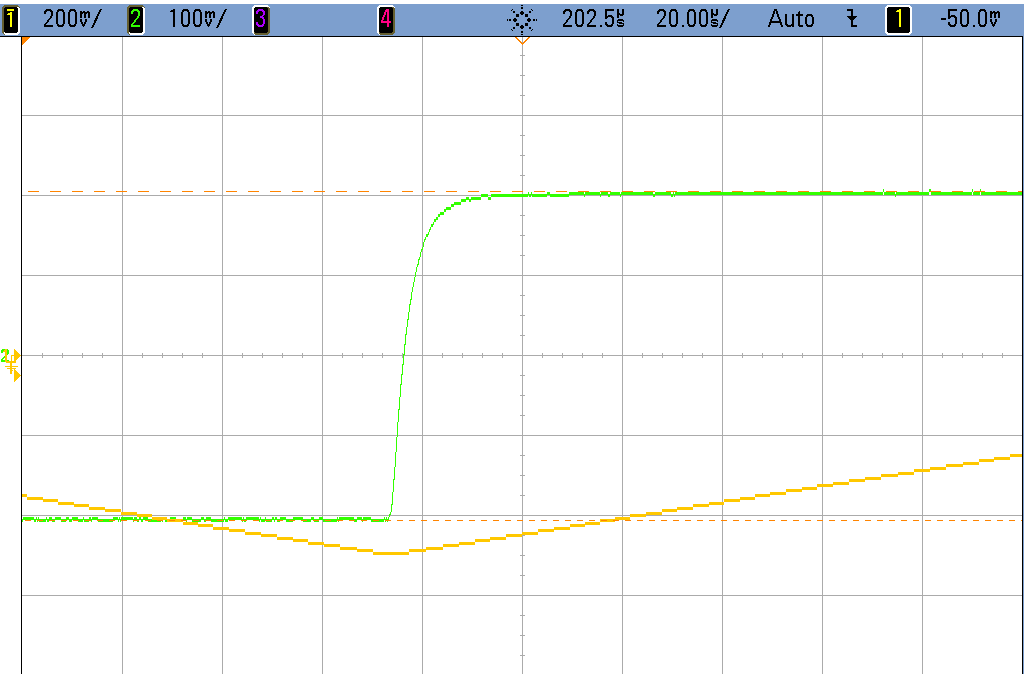
\includegraphics[scale=0.4]{fotos/tc_tp2_ej4_dcomp_1k_transitorio.png}
	\caption{Respuesta del derivador compensado (verde) a una entrada triangular (amarilla) de $1kHz$}
\end{figure}

El sistema conserva su comportamiento de derivador para frecuencias menores a $2kHz$ como se esperaba. En este caso, adem\'as, ya no se produce un \textit{overshoot} en el transitorio, si no que ahora corresponde al de un circuito de segundo orden sobreamortiguado, que es lo que pretend\'iamos al compensar el circuito.

Para frecuencias altas, sin embargo, el circuito ya no se comporta como un derivador. Esto sucede porque el per\'iodo de la se\~nal es menor que el tiempo del transitorio del circuito.

\begin{figure}  [H]
	\centering
	\label{fig:dcomp-100k}
	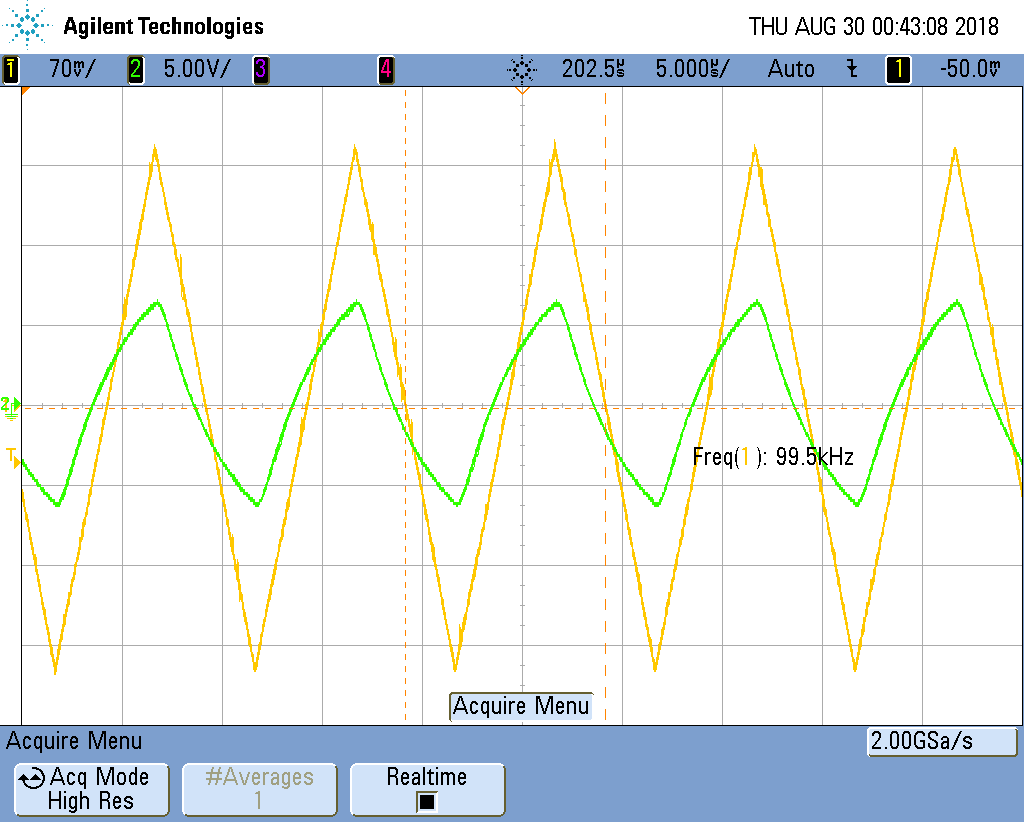
\includegraphics[scale=0.4]{fotos/tc_tp2_ej4_dcomp_100k.png}
	\caption{Respuesta del derivador compensado (verde) a una entrada triangular (amarilla) de $1kHz$}
\end{figure}



\subsection{Integrador}

Colocando los componentes en el orden inverso al derivador se obtiene el circuito integrador:


\begin{figure} [H]
	\centering
	\begin{circuitikz}
  		\draw (0,0) node[op amp] (opamp) {}
  		(opamp.-) to [R, l_=$R$, *-o] ($(opamp.-)-(2,0)$) node[left]{$V_{in}$}
  		(opamp.-) |- ($(opamp.-)+(0.2,1)$) to[C=$C$] ($(opamp.-)+(2.2,1)$) -|
  		(opamp.out) to[short,*-] ($(opamp.out)+(.5,0)$) node [right] {$V_{out}$} node [ocirc] {} 
  		(opamp.+) to[short] ($(opamp.+) - (0,.5)$) node[ground] {}
  ;
\end{circuitikz}
	\caption{Circuito integrador}
\end{figure}

\subsubsection{An\'alisis matem\'atico: respuesta en frecuencia}

 Reemplazando $Z_1$ por $R$ y $Z_2$ por $\frac{1}{sC}$ en la ecuaci\'on \ref{eq:tf-ideal}, obtenemos:


\[ H(s) =  -\frac{1}{RC\cdot s}\]

Efectuando la antitransformada de Laplace a esta expresi\'on, resulta que $v_{out}(t) = -\frac{1}{RC} \int_{-\infty}^t v(u)du$, es decir que a la salida se obtiene la integral de la se\~nal de la entrada, invertida y multiplicada por la constante $\frac{1}{RC}$. As\'i planteado, este sistema tiene ganancia infinita para corriente continua. Esto podr\'ia ser un problema debido a que cualquier ruido de frecuencias bajas se ver\'a enormemente amplificado. \par

Utilizando la ecuaci\'on \ref{eq:tf-ao}, la nueva transferencia que obtenemos es:


\[ H(s) = -  \frac {A_0}{(A_0+1)\cdot RC \cdot s+1} \]

Aqu\'i el polo se traslada del origen a $f = \frac{1}{2\pi \cdot RC \cdot (A_0+1)} \sim 5mHz$. Esto establece un m\'aximo de ganancia para continua, pero en una frecuencia tan baja que ser\'ia razonable esperar que sea un problema de todas maneras. \par

Por \'ultimo, considerando el polo del operacional la transferencia final queda en:

\begin{equation}\label{eq:tf-int} H(s) = -\frac{A_0}{\frac{RC}{\omega_p} \cdot s^2 + \left(\frac{1}{\omega_p} + (A_0+1) \cdot RC\right) \cdot s +1} \end{equation}

Esta funci\'on tiene tambi\'en un polo en $0.005Hz$, pero tiene un segundo en $16MHz$. Sin embargo, para esta frecuencia la atenuaci\'on probablemente sea tal que no se pueda medir la salida, puesto que los generadores de funciones utilizados para medir s\'olo pueden entregar hasta $20V_{pp}$. Por lo tanto, no podr\'ia en principio apreciarse un polo en esa frecuencia.


\subsubsection{An\'alisis matem\'atico: impedancia de entrada}

Idealmente, debido a la tierra virtual en $V^-$, la entrada s\'olo se carga con $Z_1 = R$, con lo cual la impedancia ser\'ia constante:

\[ Z_{in}(s) =  R\]

Si consideramos la expresi\'on \ref{zin-ao}, obtenemos en cambio que:

\[ Z_{in}(s) = \frac{(A_0+1)\cdot RC \cdot s +1}{ (A_0 +1) \cdot C \cdot s }\]

Seg\'un esta expresi\'on, tendr\'iamos un polo en el origen y un cero en $0.005Hz$. La ganancia que tendr\'ia el sistema en esas frecuencias ser\'ia, sin embargo, tan elevada que impidir\'ia medir la entrada sin que la salida sature, con lo cual s\'olo se podr\'ia medir en frecuencias donde los efectos del polo y el cero ya fueron neutralizados entre s\'i, y la expresi\'on se ver\'ia nuevamente reducida a $Z_{in}=R$.\par

Finalmente, con el modelo de $A_{vol}$ la impedancia de entrada resulta ser:

\begin{equation}Z_{in}(s) = \frac{\frac{RC}{\omega_p} \cdot s^2 + \left(\frac{1}{\omega_p} + (A_0+1) \cdot RC\right) \cdot s +1}{sC \cdot (A_0+1) \cdot \left(\frac{1}{\omega_p (A_0+1)}\cdot s +1\right) } \end{equation}

Los polos de la transferencia mencionados en \ref{eq:tf-int} son ahora ceros de la impedancia. Esta funci\'on cuenta tambi\'en con un polo en $f = \frac{omega_p(A_0+1)}{2\pi} \sim BWP = 16MHz$ , que es la misma frecuencia de uno de los ceros. Esto implica que sus efectos se ven cancelados entre s\'i, quedando s\'olo el cero en $0.005Hz$.




\subsubsection{An\'alisis de resultados: respuesta en frecuencia}

\begin{figure}  [H]
	\centering
	\label{fig:i-hf}
	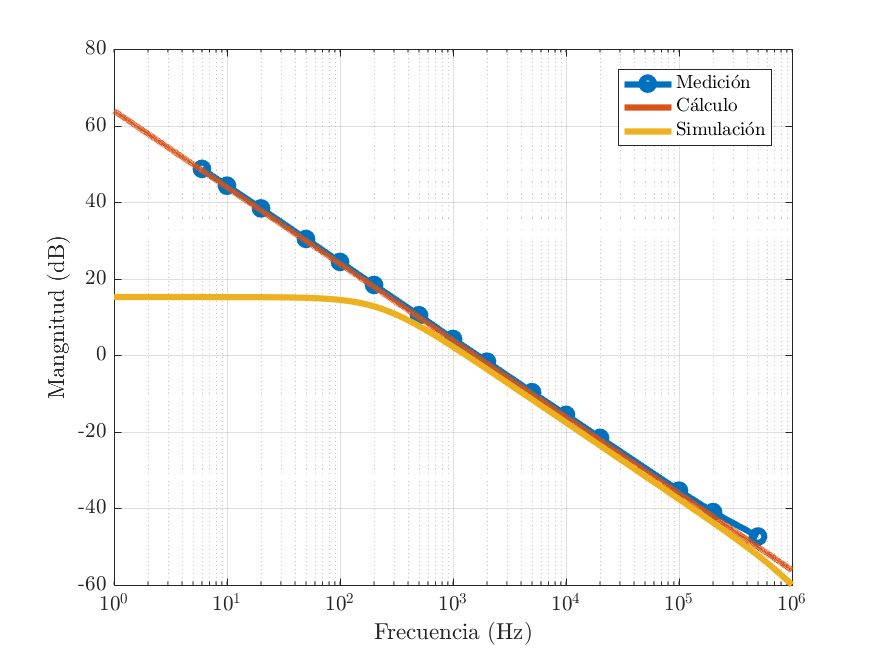
\includegraphics[scale=0.7]{fotos/tc_tp2_ej4_i_Hf_mag.png}
	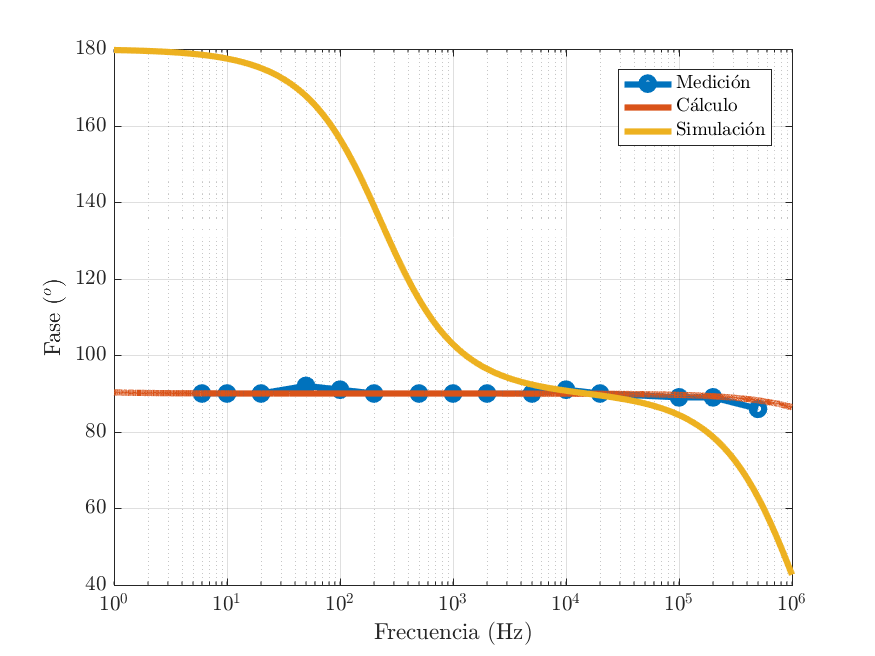
\includegraphics[scale=0.7]{fotos/tc_tp2_ej4_i_Hf_fase.png}
	\caption{Respuesta en frecuencia del integrador}
\end{figure}

El circuito se comporta como un integrador ideal en el rango de frecuencias donde se midi\'o. Para frecuencias m\'as bajas la saturaci\'on del operacional debido a la alta ganancia del circuito impidi\'o realizar m\'as mediciones. No se explica por qu\'e el simulador obtiene resultados tan dispares con los obtenidos te\'oricamente, si bien a partir de los $100Hz$ el comportamiento de la magnitud es el de un polo simple.




\subsubsection{An\'alisis de resultados: impedancia de entrada}

\begin{figure}  [H]
	\centering
	\label{fig:i-zin}
	\includegraphics[scale=0.7]{fotos/tc_tp2_ej4_i_zin_mag.png}
	\includegraphics[scale=0.7]{fotos/tc_tp2_ej4_i_zin_fase.png}
	\caption{Impedancia de entrada del integrador}
\end{figure}

Hasta aproximadamente $100kHz$, el comportamiento del circuito se corresponde con el modelo ideal, es decir, una resistencia de aproximadamente $15k\Omega$ con fase $0^\circ$. En frecuencias m\'as elevadas, sin embargo, aparece un polo de primer orden en $500kHz$ cuya presencia no se explica ni con el modelo de $A_{vol}(s)$, ni agregando la capacidad par\'asita entre $V^+$ y $V^-$ de $12pF$, ni agregando las puntas del osciloscopio.


\subsubsection{An\'alisis de resultados: respuesta transitoria}
Seg\'un lo osbservado en la respuesta en frecuencia, el circuito deber\'ia poder integrar se\~nales de todas las frecuencias que se midieron. Efectivamente, no se logr\'o medir ninguna se\~nal que no se integrara dentro del rango de frecuencias donde la salida no estaba demasiado atenuada para ser medida ni demasiado amplificada como para no poder medir la entrada.  A continuaci\'on se ilustra uno de los casos medidos, donde se observa que la salida de una constante es una lineal, es decir su integral:

\begin{figure}  [H]
	\centering
	\label{fig:i-1k}
	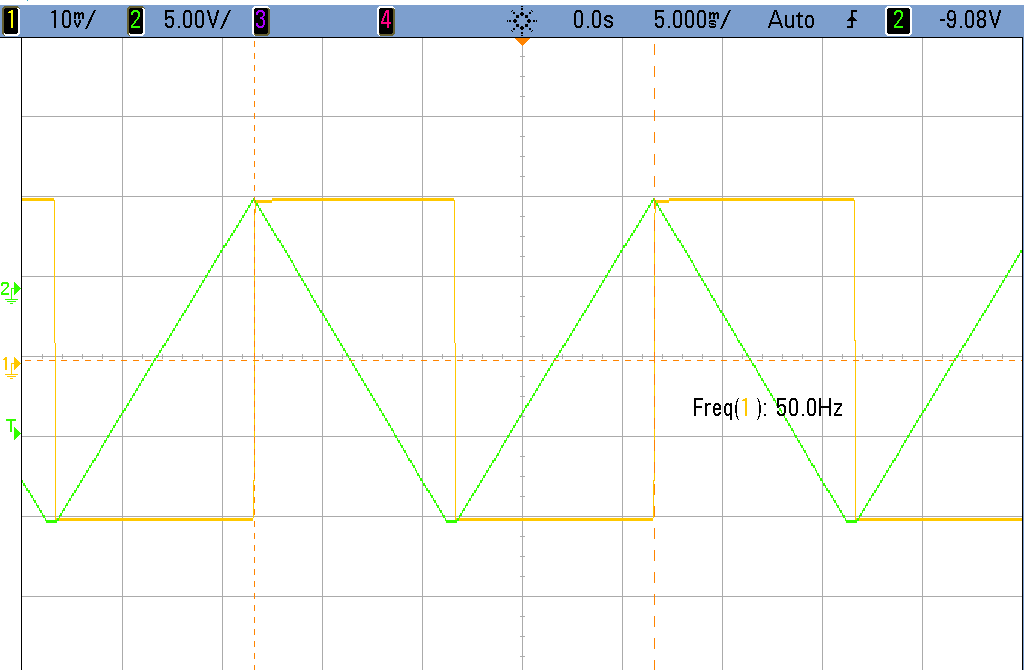
\includegraphics[scale=0.4]{fotos/tc_tp2_ej4_i_50.png}
	\caption{Respuesta del integrador (verde) a una entrada de tren de pulsos (amarilla) de $1kHz$}
\end{figure}





\subsection{Integrador compensado}

Como ya se mencion\'o, el circuito integrador ideal tiene un polo en el cero. Esto implica que el circuito tiene, en teor\'ia, ganancia infinita en continua. Efectivamente, cuanto m\'as disminu\'ia la frecuencia en el caso anterior m\'as dif\'icil se hac\'ia medir, puesto que entradas de amplitud muy peque\~nas saturaban el \textit{op amp}. A su vez, constantemente se deb\'ia ajustar el \textit{offset} del generador para compensar la corriente continua par\'asita que aparec\'ia en el circuito, pues esto ocasionaba que la se\~nal de salida saturara hasta quedar continua en $V_{out} \sim V_{cc}$. \par

Para compensar esta situaci\'on, se busca correr el polo del origen lo suficiente como para que en frecuencias bajas llegue a un m\'aximo razonable. Como se explicar\'a anal\'iticamente a continuaci\'on, esto puede lograrse colocando una resistencia en paralelo con el capacitor. A grandes rasgos, esto evita que el circuito funcione en \textit{open loop} cuando el capacitor se abre por la baja frecuencia, ya que hay un m\'inimo de impedancia constante.

\begin{figure} [H]
	\centering
	\begin{circuitikz}
	
  		\draw (0,0) node[op amp] (opamp) {}
  		(opamp.-) to [R, l_=$R$, *-o] ($(opamp.-)-(2,0)$) node[left]{$V_{in}$}
  		(opamp.-) |- ($(opamp.-)+(0.2,1)$) to[C=$C$] ($(opamp.-)+(2.2,1)$) -|
  		(opamp.out) to[short,*-] ($(opamp.out)+(.5,0)$) node [right] {$V_{out}$} node [ocirc] {} 
  
  		 ($(opamp.-)+(0.2,1)$)  
  		 to [short, *-] ($(opamp.-)+(0.2,3)$) 
		to [R,  l_=$R_C$, *-] ($(opamp.-)+(2.2,3)$) 
 		to  [short, *-]($(opamp.-)+(2.2,1)$)
 		
 		(opamp.+) to[short] ($(opamp.+) - (0,.5)$) node[ground] {}
  ;
	\end{circuitikz}
	\caption{Circuito integrador compensado}
\end{figure}



\subsubsection{An\'alisis de matem\'atico}
La configuraci\'on de este circuito es $Z_1 = R$ y $Z_2 = (s\cdot C + \frac{1}{R_C})^{-1} = \frac{R_C}{s\cdot R_C C + 1}$, donde llamaremos $R_C$ a la resistencia de compensaci\'on. Puesto que el circuito integrador quedaba aptamente descripto por el modelo ideal para su respuesta en frecuencia, calcularemos el valor de $R_C$ seg\'un este modelo.\par

Reemplazando en la ecuaci\'on gen\'erica por los valores mencionados, la transferencia ideal del circuito resulta:

\[ H(s) = - \frac{R_C}{R_1} \cdot \left(\frac{1}{s \cdot RC + 1}\right)\]

La ganancia se obtiene, entonces, tomando $\lim_{f\to 0^+} \abs{H(i2\pi f)} = \frac{R_C}{R_1}$. Teniendo en cuenta que esta ser\'a la amplificaci\'on del ruido de se\~nales de baja frecuencia, donde el sistema no podr\'a integrar, tomaremos como criterio que esta ganancia sea $6dB$, es decir que $R_C \sim 2 \cdot R_1 = 30k\Omega$. El valor comercial elegido es entonces $R_C = 27k\Omega$. El cero queda posicionado entonces en $f = \frac{1}{2\pi \cdot R_C C} \sim 870Hz$. \par

La impedancia de entrada ideal es la misma que se obtiene en el integrador no compensado.\par

Las f\'ormulas de $H(s)$ y $Z_{in}(s)$ para el modelo $A_0$ finito y con polo dominante se obtienen de forma an\'aloga a como se oper\'o hasta el momento: reemplazando los valores de $Z_1$ y $Z_2$ en la expresiones gen\'ericas por los de este circuito. Sin embargo, como no aportaron informaci\'on que afectara lo medido en el caso del integrador (y como se ver\'a m\'as adelante, tampoco en este), no se incluir\'an. 






\subsubsection{An\'alisis de resultados: respuesta en frecuencia}

\begin{figure}  [H]
	\centering
	\label{fig:icomp-hf}
	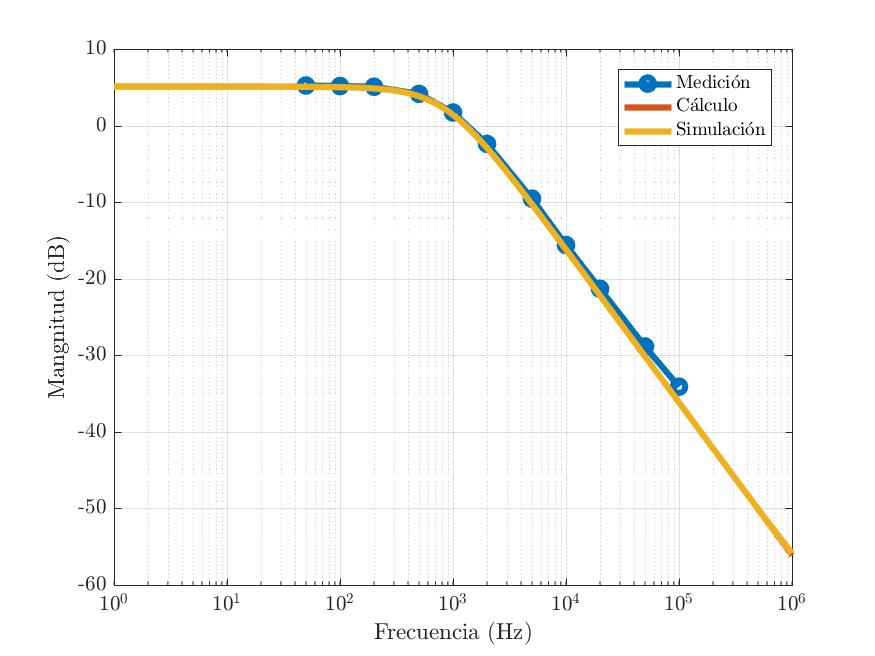
\includegraphics[scale=0.7]{fotos/tc_tp2_ej4_icomp_Hf_mag.png}
	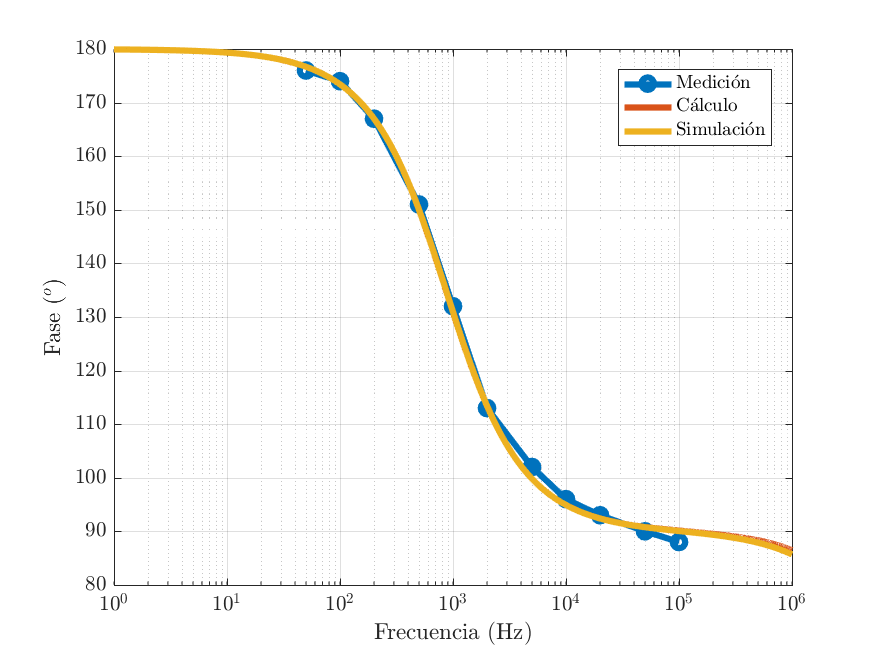
\includegraphics[scale=0.7]{fotos/tc_tp2_ej4_icomp_Hf_fase.png}
	\caption{Respuesta en frecuencia del integrador compensado}
\end{figure}

Los resultados obtenidos con el simulador y con la teor\'ia son tan similares que no logran distinguirse en el gr\'afico. Las mediciones tambi\'en quedaron en l\'inea con lo predicho por ambos modelos. Cabe aclarar que la funci\'on utilizada para el c\'alculo te\'orico es la de utiliza $A_{vol}(s)$, pero sin embargo el comportamiento no se distingue de un sistema con un polo simple en $f \sim 900Hz$.


\subsubsection{An\'alisis de resultados: impedancia de entrada}

\begin{figure}  [H]
	\centering
	\label{fig:icomp-zin}
	\includegraphics[scale=0.7]{fotos/tc_tp2_ej4_icomp_zin_mag.png}
	\includegraphics[scale=0.7]{fotos/tc_tp2_ej4_icomp_zin_fase.png}
	\caption{Impedancia de entrada del integrador compensado}
\end{figure}

En este caso, se observa un polo de primer orden en $f=500kHz$.  Esto no corresponde con ninguno de los modelos planteados ni se puede explicar agregando las puntas ni la \textit{differential input capacitance}. Sin embargo, el comportamiento inicial es el de una resistencia de $\sim 15k\Omega$, que era lo que se esperaba obtener. Tambi\'en en este caso se est\'a utilizando la expresi\'on de $Z(s)$ con $A_{vol}(s)$ para el c\'alculo te\'orico.

\subsubsection{An\'alisis de resultados: respuesta transitoria}

Al correr el polo del origen a $900Hz$, el circuito deja de integrar en se\~nales de frecuencia de este orden de magnitud o menores, puesto que hasta ese punto se comporta como constante (predomina la resistencia).
\begin{figure}  [H]
	\centering
	\label{fig:i-1k}
	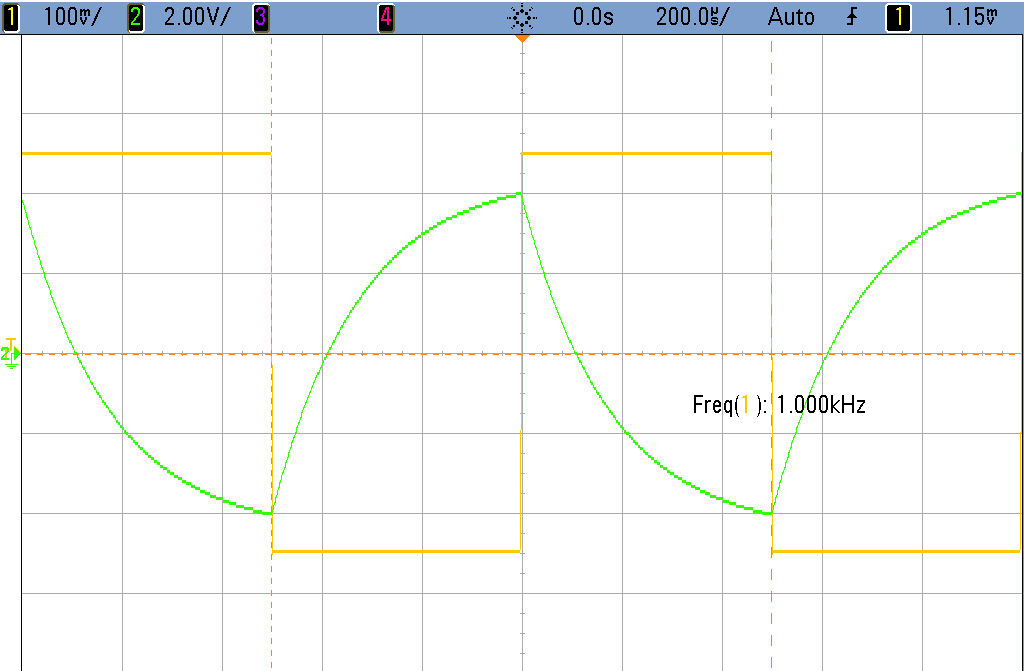
\includegraphics[scale=0.4]{fotos/tc_tp2_ej4_icomp_1k.png}
	\caption{Respuesta del integrador compensado (verde) a una entrada de tren de pulsos (amarilla) de $1kHz$}
\end{figure}

Cuando la frecuencia es mucho mayor que la de corte, en cambio, el t\'ermino constante se hace despreciable y la transferencia se puede aproximar con la de un integrador ideal. Entonces, podemos observar en la salida la integral de la entrada.

\begin{figure}  [H]
	\centering
	\label{fig:i-1k}
	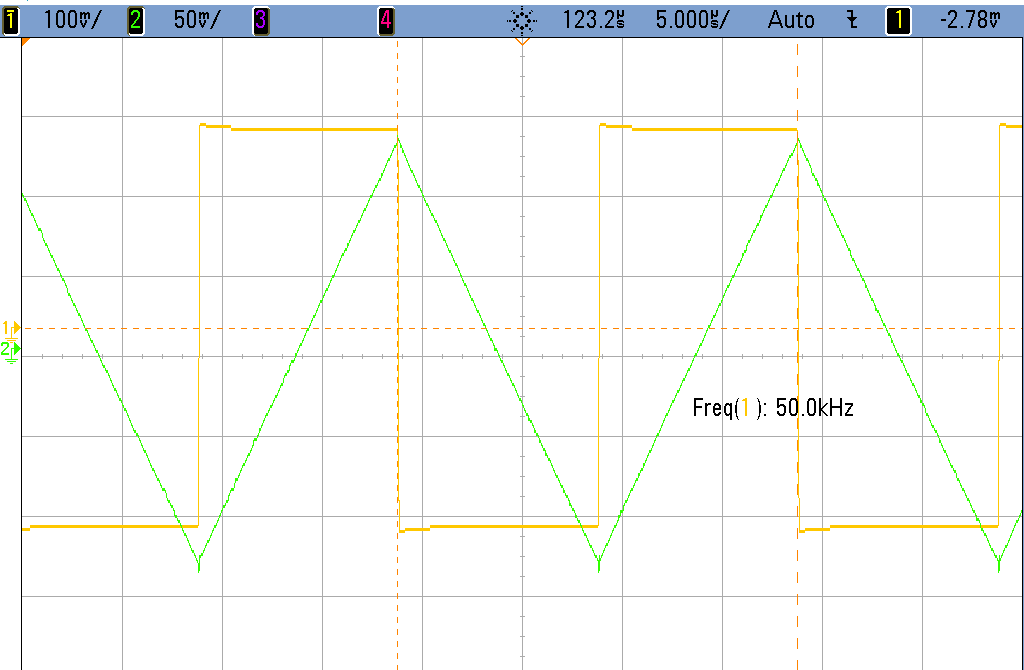
\includegraphics[scale=0.4]{fotos/tc_tp2_ej4_icomp_50k.png}
	\caption{Respuesta del integrador compensado (verde) a una entrada de tren de pulsos (amarilla) de $50kHz$}
\end{figure}




\subsection{Conclusiones}
Si bien los circuitos no compensados cumplen su funci\'on de integrador y derivador en un amplio rango de frecuencias, ambos traen problemas a la hora de utilizarlos.\par

En el caso del derivador, debido a la interacci\'on entre los polos del operacional con el resto del circuito se form\'o un sistema de segundo orden subamortiguado. Esto provoca picos de tensi\'on en la respuesta transitoria y ganancia de m\'as de $40dB$ en la frecuencia del polo, lo cual lo hace inutilizable en este rango de frecuencias. Al compensar este efecto con una resistecia en serie, limitando la impedancia de entrada para que no se haga 0 cuando el capacitor pasa a comportarse como un cable, el sistema pas\'o de estar subamortiguado a sobreamortiguado, con lo cual estos problemas se vieron solucionados. Sin embargo, el rango de frecuencias donde el circuito derivaba se redujo al de mucho menores que la frecuencia de corte. Elegir una resistencia de compensaci\'on menor habr\'ia ampliado este rango unos $kHz$ m\'as, pero a costo de tener m\'as ganancia entre el primer polo y el segundo.\par

En cuanto al integrador, fue necesario limitar la ganancia en frecuencias bajas para que \textit{offsets} de unos pocos milivolt en la entrada de continua no deseada saturaran el operacional. Al compensar este problema, sin embargo, el circuito dej\'o de integrar para frecuencias menores o del mismo orden que la del nuevo polo.\par


\end{document}
